Les lignes DC sont connectées par des prises \uD, à part au passage câbles bleus $\rightarrow$ Manganin.

On utilise les 17 lignes intérieures, c'est-à-dire pas les 4 coins de la prise.

\subsection{Soudure des prises uD}
Les prises \uD sont assez fragiles, il ne faut pas appuyer trop sur les pins avec le fer, au risque de les casser (rattrapable mais pas très pratique). La technique est de remplir la pin d'étain, puis de glisser le fil dedans sans avoir à apporter d'étain.

Il est préférable de mettre une gaine thermorétractable à une soudure sur deux (j’ai aussi mis de la grosse gaine thermo pour isoler les deux lignes).


\subsection{Presses de thermalisation}
À l'étage 100mK, on thermalise les câbles de manganin à l'aide de la (double) presse dorée. On colle le tout à l'aide de Stycast :
\begin{description}
    \item[Résine] Stycast (Emerson \& Cuming) 1kg
    \item[Durcisseur] Stycast (Emerson \& Cuming) 12g
\end{description}
Il faut utiliser $8\%$ de durcisseur dans le mélange.

Il faut faire attention aux câbles qui se superposent : cela peut rendre le contact thermique mauvais pour l'ensemble des câbles.

On utilise une batterie au plomb pour faire poids pendant quelques heures.

\subsection{Boîtier de thermalisation}
Voilà.

\subsection{Tresse}
Entre les boîtiers de thermalisation et de filtrage, les câbles bleus sont blindés par une tresse d'aluminium. Il est préférable de faire passer les câbles une fois qu'une (seule) prise \uD est soudée.

Cette tresse sera soudée sur les prises \uD et maintenue grâce à des plaques métalliques afin de la thermaliser.

\subsection{Boîtier de filtrage}
Afin de filtrer les micro-ondes des lignes DC, nous faisons passer les 17 câbles par un boîtier rempli d'Écosorb.

On utilise 17 câbles bleus de 80cm (faible résistivité). Ces câbles sont entortillés autour d'une chute de câble coaxial. On les passe alors d'abord dans les pièces en PLA puis on les soude sur les prises \uD.

\subsubsection{Connexions du bloc}
Le bloc est connecté grâce à des prises \uD. Les vis d'entrée sont "maison", les vis de sortie sont des vis Allen 2.5mm. Faire attention à l'orientation de la prise de sortie en fonction de la prise correspondante sur la canne du porte-échantillon.

\subsubsection{Compartimentage du bloc}
Malheureusement, l'Écosorb peut abîmer les soudures et les câbles au bout de quelques cycles de refroidissement. Nous avons donc décidé de compartimenter ce boîtier pour protéger les connexions.

Des pièces en PLA vont alors être imprimées. Elles ont été dessinées grâce à OpenSCAD et converties au format STL. On peut trouver tout ça sur mon dépôt Git.

\begin{figure*}[t!]
    \centering
    \begin{subfigure}[t]{0.59\textwidth}
        \centering
        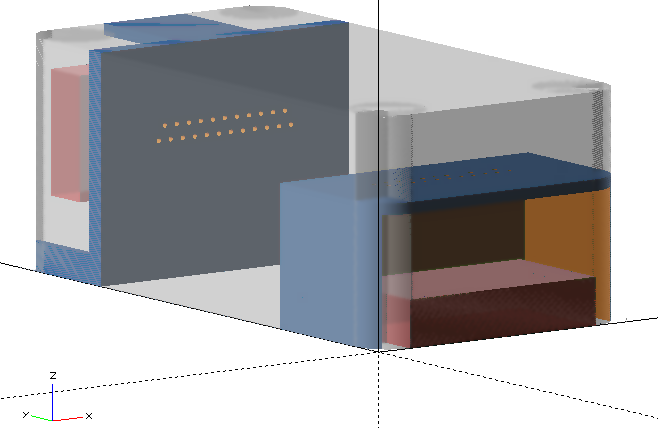
\includegraphics[height=0.633\textwidth]{Images/Thermalisation/Filtrage3D}
        \caption{Modélisation 3D des pièces dans le boîtier}
    \end{subfigure}%
    ~ 
    \begin{subfigure}[t]{0.39\textwidth}
        \centering
        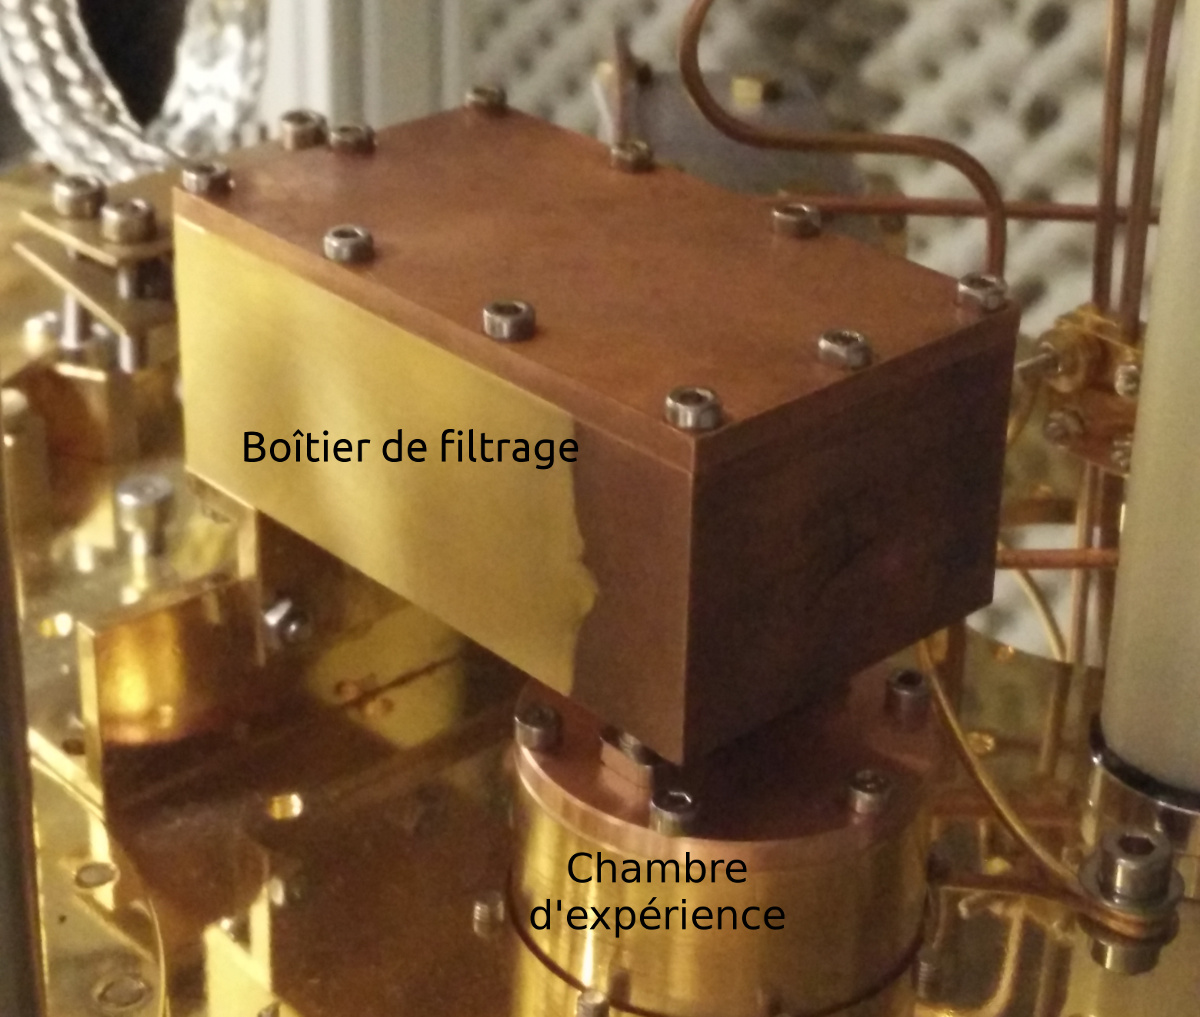
\includegraphics[height=0.95\textwidth]{Images/Thermalisation/Filtrage}
        \caption{Boîtier de filtrage en place dans le cryostat}
    \end{subfigure}
    \caption{Boîtier de filtrage, rempli d'Eccosorb}
\end{figure*}

\subsubsection{Préparation de l'Écosorb}
\begin{description}
    \item[Résine] Eccosorb (Emerson \& Cuming) CRS 117 PTA 1kg
    \item[Durcisseur] Eccosorb (Emerson \& Cuming) CRS PTB 12g
\end{description}
Il faut utiliser $1,18\%$ de durcisseur dans le mélange.

Ici on a mélangé 2,5g de catalyseur pour 212g de pâte. Il faut d'abord bien homogénéiser la résine (A) avant de mélanger au durcisseur (B).

Le mélange sèche en quelques jours. Il faut donc faire attention à poser le bloc bien à l'horizontale (en pensant aux prises) et à l'abri.


\begin{BOM}
    \item 10 \fois Vis M2
    \item 2 \fois Prises \uD femelle
    \item 4 \fois Vis M1 + écrou + 2 rondelles (pour les prises)
\end{BOM}

\subsection{Connexion avec la canne}
On utilise une prise \uD (vis maison) que l'on fixe sur le bouchon de la canne. \emph{Faire attention au sens de branchement}, en fonction de l'aménagement du cryostat (des traits au feutre noir indiquent le sens sur ce que j'ai fait).

Le boîtier cylindrique et son couvercle (à fixer après la prise…) sont vissés par des vis M2. Les lignes sont ensuite connectées par des barrettes au porte-échantillon.

\begin{BOM}
    \item 0 \fois Vis M2
    \item 1 \fois Prise \uD mâle
    \item 17 \fois Barette de connexion
\end{BOM}

